
\documentclass[10pt]{beamer}
\usepackage{kotex}
\usepackage{ulem}

\usepackage{framed}
\usepackage{graphicx}
%https://www.overleaf.com/learn/latex/Inserting_Images

\usepackage{amsmath}
%use dfrac
\usepackage{xcolor}

\usepackage{amsthm}
%\usepackage{tabl}
\usepackage{listings}
\definecolor{mGreen}{rgb}{0,0.6,0}
\definecolor{mGray}{rgb}{0.5,0.5,0.5}
\definecolor{mPurple}{rgb}{0.58,0,0.82}
\definecolor{backgroundColour}{rgb}{0.95,0.95,0.92}
%https://tex.stackexchange.com/questions/348651/c-code-to-add-in-the-document
\lstdefinestyle{CppStyle}{
    backgroundcolor=\color{backgroundColour},   
    commentstyle=\color{mGreen},
    keywordstyle=\color{magenta},
    numberstyle=\tiny\color{mGray},
    stringstyle=\color{mPurple},
    basicstyle=\footnotesize,
    breakatwhitespace=false,         
    breaklines=true,                 
    captionpos=b,                    
    keepspaces=true,                 
    numbers=left,                    
    numbersep=5pt,                  
    showspaces=false,                
    showstringspaces=false,
    showtabs=false,                  
    tabsize=2,
    language=C++
}

\usepackage{url}

\usepackage{etoolbox}
\AtBeginEnvironment{quote}{\singlespacing\small}


\usepackage{thmtools}
\usepackage{xcolor}
\declaretheoremstyle[% spaceabove=6pt,spacebelow=6pt, headfont=\color{MainColorOne}\sffamily\bfseries, notefont=\mdseries, notebraces={[}{]}, bodyfont=\normalfont,
headpunct={},
postheadspace=1em,
%qed=▣,
]{maintheorem}

\declaretheorem[%
name=정의,
style=maintheorem,
numberwithin=section, shaded={%bgcolor=MainColorThree!20,
margin=.5em}]{dfn}
% \begin{dfn}[]
% \end{dfn}

\setbeamertemplate{footline}[frame number]

%\usetheme{Hannover}
\usetheme{CambridgeUS}


\title{기초알고리즘, 분할정복 (divide and conquer)}

\author{EUnS}

\begin{document}


\begin{frame}{}
    \maketitle
\end{frame}    



\begin{frame}[fragile]{}
    \begin{lstlisting}[style = CppStyle]
    INSERTION-SORT(A)
    for j = 2 to A.length
        key = A[j]
        // Insert A[j] into the sorted sequence A[1 .. j - 1].
        i = j - 1
        while i > 0 and A[i] > key
            A[i + 1] = A[i]
            i = i - 1
        A[i + 1] = key
    \end{lstlisting}
\end{frame}


\begin{frame}{시간복잡도}
    \begin{itemize}
        \item 최악의 경우 시간 복잡도 \pause
        $$\Theta(n^2)$$
        \item 최선의 경우 시간 복잡도  \pause
        $$\Theta(n)$$
        \item 평균 시간 복잡도
        $$\Theta(n^2)$$
    \end{itemize}
\end{frame}




\begin{frame}{시간복잡도}
    \begin{itemize}
        \item if에 의해서 정확하게 구하기 어렵다. \pause
        \item 입력 자료의 상태에 따라 시간 복잡도는 바뀐다. \pause
        \item 최악은 for문만을 가지고 단순 계산해도 무방. \pause
        \item ps에선 1초에 $10^9$(1억번)정도 계산한다고 생각하고 어림잡아 계산.
    \end{itemize}
\end{frame}



% \begin{frame}{}
%     \tableofcontents
% \end{frame}   

\begin{frame}{분할정복}
    문제를 세가지 단계를 거치면서 재귀적으로 문제를 푼다.
    \begin{enumerate}
        \item 분할 : 현재의 문제와 동일하되 입력의 크기가 더 작은 다수의 부분 문제로 분할한다.
        \item 정복 : 부분 문제를 재귀적으로 풀어서 정복. 부분 문제의 크기가 충분히 작으면 직접적인 방법으로 푼다.
        \item 결합 : 부분 문제의 해를 결합해 원래 문제의 해가 되도록 만든다.
    \end{enumerate}
\end{frame}



\begin{frame}{분할정복 예시}
    \begin{itemize}
        \item 머지소트
        \item 최대부분 배열문제를 해결하는 알고리즘
        \item 퀵소트
        \item 행렬 곱
        \item FFT
        \item 카라추바 알고리즘
    \end{itemize}
\end{frame}



\begin{frame}{분할정복 예시}
    \begin{itemize}
        \item 머지소트
        \item 최대부분 배열문제를 해결하는 알고리즘
        \item 퀵소트
        \item \sout{행렬 곱}
        \item \sout{FFT}
        \item \sout{카라추바 알고리즘}
    \end{itemize}
\end{frame}





\begin{frame}{최대 부분 배열문제(Maximum subarray problem)}
    \begin{itemize}
        \item 배열값중 구간 끝값의 차가 가장 큰 구간 찾기
    \end{itemize}
    \begin{figure}[h!]
        %\centering
        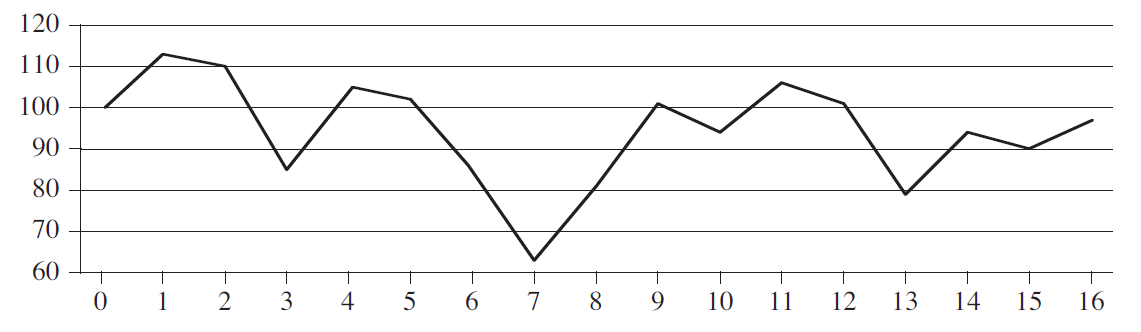
\includegraphics[scale=0.25]{subarray.png}
    \end{figure}
\end{frame}


\begin{frame}{해}
    \begin{figure}[h!]
        %\centering
        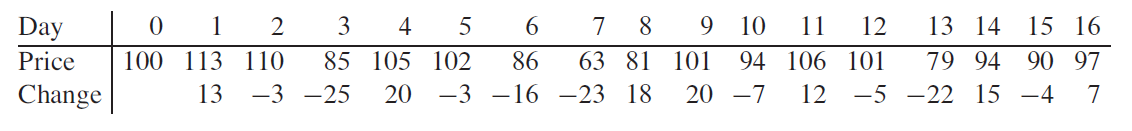
\includegraphics[scale=0.4]{table.png}
    \end{figure}

    \begin{itemize}
        \item 주먹구구
        과제로 만들어올것.
    \end{itemize}
\end{frame}


\begin{frame}{분할정복을 이용한 방법}
    \begin{itemize}
        \item 인덱스 low... high 사이의 임의의 mid를 잡고 이 중 최대 부분 배열이 어디에 속하는지 생각해보자.  \pause
        \item low ,mid 사이 \pause
        \item mid high 사이 \pause
        \item mid를 걸치는 low high 사이 \pause
        \item 이것이 분할의 세가지 케이스
    \end{itemize}
\end{frame}

\begin{frame}{분할정복을 이용한 방법}
    \begin{itemize}
        \item 분할 : 일단 전체 길이를 반으로 쪼갠다. \pause
        \item 정복 : 상수시간. \pause
        \item 결합 : 걸쳐있는 경우 좌우 길이를 새로 구하고 각각의 길이를 리턴한뒤 비교한다.
    \end{itemize}
\end{frame}


\begin{frame}[fragile]{분할정복을 이용한 방법}
    \begin{lstlisting}[style = CppStyle]
    FIND-MAXIMUM-SUBARRAY(A, low, high)
    if high == low
        return (low, high,A[low]) // base case: only one element
    else mid = (low + high)/2 
        (left-low, left-high, left-sum) 
            = FIND-MAXIMUM-SUBARRAY(A, low, mid)
        (right-low, right-high, right-sum) 
            = FIND-MAXIMUM-SUBARRAY(A, mid + 1, high)
        (cross-low, cross-high, cross-sum) 
            = FIND-MAX-CROSSING-SUBARRAY(A, low, mid, high)

        if left-sum >= right-sum and left-sum >= cross-sum
            return (left-low, left-high, left-sum)
        elseif right-sum >= left-sum and right-sum >= cross-sum
            return (right-low, right-high, right-sum)
        else return (cross-low, cross-high, cross-sum)
    \end{lstlisting}
\end{frame}    

\begin{frame}[fragile]{분할정복을 이용한 방법}
    \begin{lstlisting}[style = CppStyle]
    FIND-MAX-CROSSING-SUBARRAY(A, low, mid, high)
    left-sum = -inf
    sum = 0
    for i = mid downto low
        sum = sum + A[i]
        if sum > left-sum
            left-sum = sum
            max-left = i
            right-sum = -inf
    sum = 0
    for j = mid + 1 to high
        sum = sum + A[j ]
        if sum > right-sum
            right-sum = sum
            max-right = j
    return (max-left, max-right, left-sum + right-sum)
    \end{lstlisting}
\end{frame}    

\end{document}

% \stop




\begin{frame}{}
    \href{}{\textcolor{blue}{참고}}
\end{frame}    

% \begin{frame}{}
%     \begin{figure}[h!]
%         %\centering
%         \includegraphics[scale=0.25]{}
%         \caption{}
%     \end{figure}
% \end{frame}    

